%-------------------------------------------------------
\begin{frame}{Raw Data}{What is the nature of the raw material? How can we use it?}
%-------------------------------------------------------

\begin{itemize}

    \item<1->\textbf{Data about \alert{students}}: \emph{anonymous students records} about academic career results, in a certain time span: \\
        \noindent\begin{centering}
            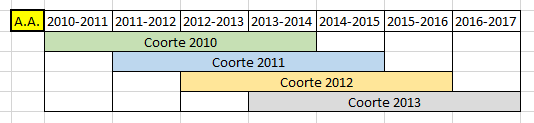
\includegraphics[scale=0.50]{../raw/stud_comp.png}
        \end{centering}

    \vspace{0.2cm}

    \item<2->\textbf{Data about \alert{courses}}: teachings evaluations questionaries compiled by the students, in an \emph{aggregate form}, about those Academical Years: \\ \vspace{0.1cm}
        \hspace{0.6cm}\textcolor{cyan}{\texttt{2010-2011, 2011-2012, \ldots, 2016-2017}}

\end{itemize}

\end{frame}

%-------------------------------------------------------
\begin{frame}{Students Data Understanding}{Example of visualization technique: interpreting a scatter plot}

    \vspace{0.2cm}
    \begin{centering}
        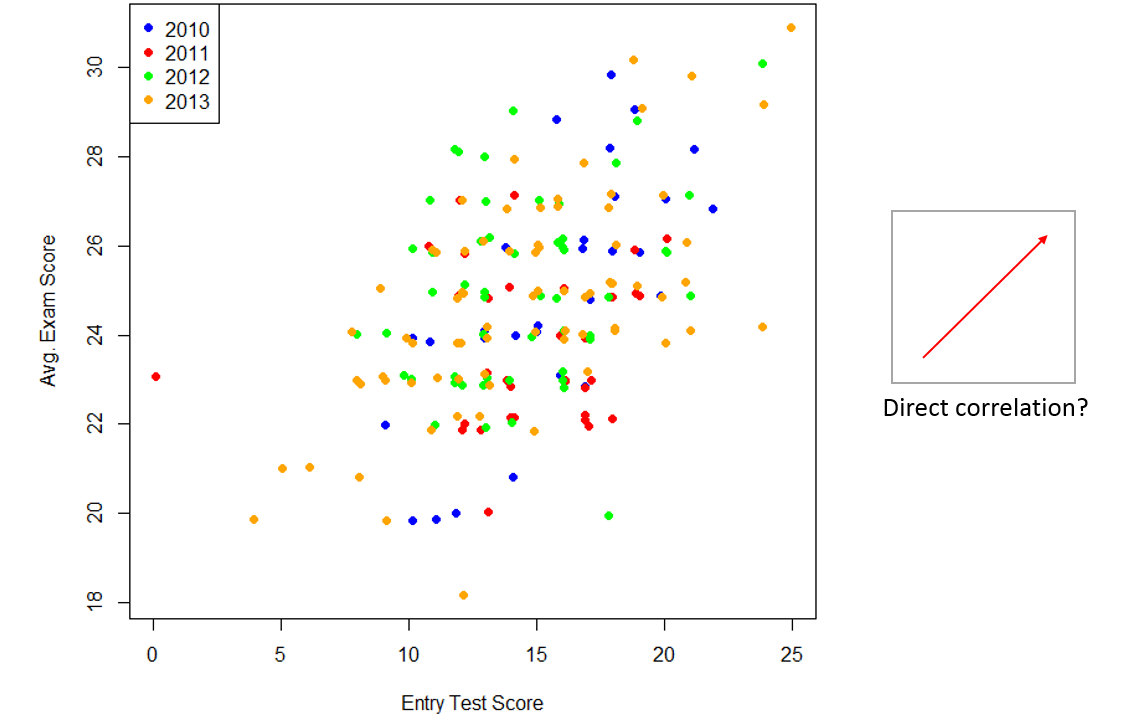
\includegraphics[scale=0.28]{img2_noback.png}
    \end{centering}

\end{frame}

\begin{frame}{Students Data Understanding}{Interpreting a std. dev. matrix about first year exam scores}

    \vspace{0.25cm}
    \noindent\begin{centering}
        \hspace{-1cm}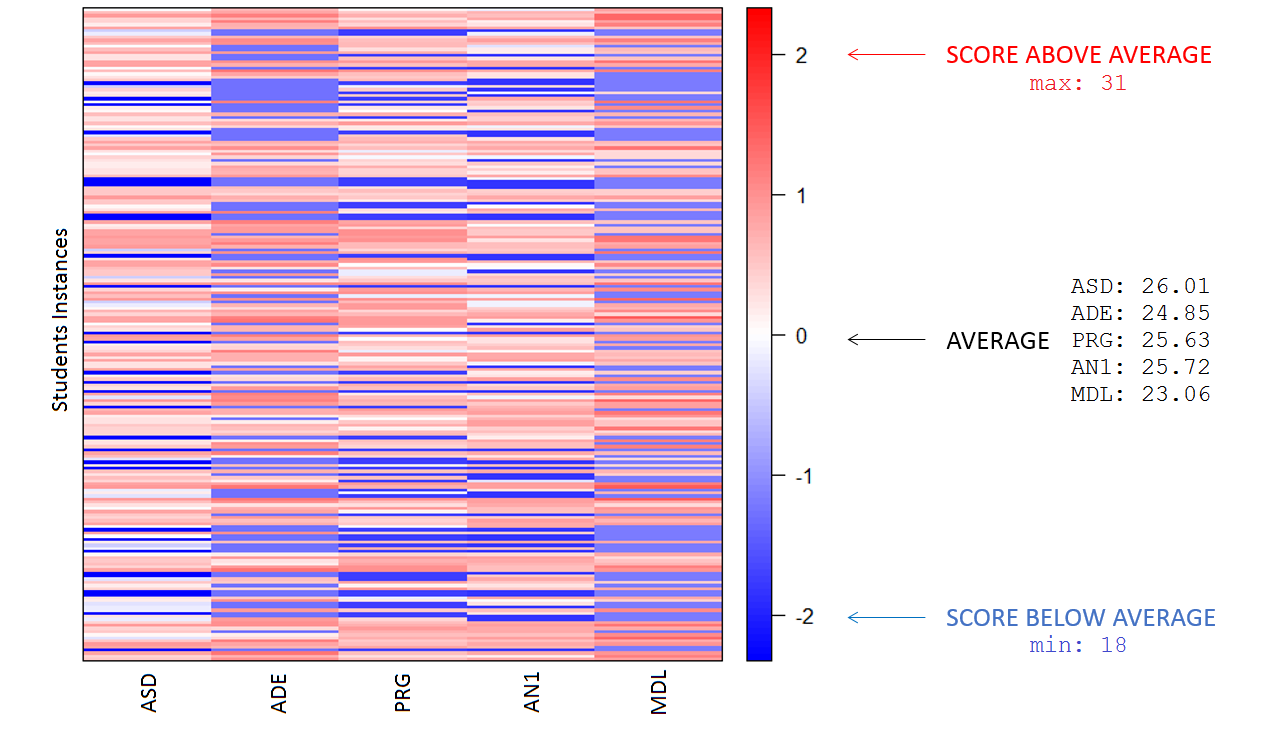
\includegraphics[scale=0.38]{img3.png}
    \end{centering}

\end{frame}
